\documentclass[12pt,t]{beamer}
\usepackage[utf8]{inputenc}
\usepackage[T1]{fontenc}
\usepackage[english]{babel}
\usepackage{pslatex}
\usepackage{mdwlist}
\usepackage{graphicx}
\usepackage{wrapfig}
\usepackage{caption}
\usepackage{subcaption}
\usepackage{float}
\usepackage{pgfgantt}

\newcommand{\tocframe}{\begin{frame}
    \frametitle{Table of Contents}
    \tableofcontents[currentsection,currentsubsection]
\end{frame}}

\newcommand{\graphicc}[4]{\begin{figure}[H] \centering
            \includegraphics[width={#1\textwidth}, keepaspectratio=true]{{#2}}
            \caption{{#3}} \label{#4} \end{figure}}

\usetheme[unit=ics]{Frederiksberg}
\title{Bachelor Project}
\subtitle{Visualizing Chan-Vese segmentation results through the DSC framework
in Autodesk Maya}
\author{Martin Jørgensen}


\begin{document}
\frame[plain]{\titlepage}

\section{Introduction}
\tocframe

\begin{frame}
    \frametitle{Introduction}
    \vspace*{\fill}
    Designing a cross-platform solution to visualize the result of
    the given Chan-Vese simulation using the DSC framework via a plugin for
    Autodesk Maya.
    \vspace*{\fill}
\end{frame}


\section{Theory}
\tocframe


\subsection{DSC}
\begin{frame}
    \frametitle{Deformable Simplical Complexes}
    \framesubtitle{Theory}

    \begin{columns}
      \begin{column}{0.48\textwidth}
        \begin{itemize}
          \item Simplical Complexes
          \item Criteria
          \item Domains
          \item Quality measure
        \end{itemize}
      \end{column}
      \begin{column}{0.48\textwidth}
        \graphicc{0.8}{img/domains.png}{Image from
          \url{http://doc.cgal.org/}}{fig:domains}
      \end{column}
    \end{columns}

\end{frame}

\subsection{Chan-Vese}
\begin{frame}
    \frametitle{Chan-Vese Segmentation}
    \framesubtitle{Theory}

    \begin{columns}
      \begin{column}{0.48\textwidth}
        \begin{itemize}
          \item Level-Set Method
          \item Adapted Chan-Vese Method
        \end{itemize}
        {\tiny \begin{align*}
  \text{Ê}(C) = &\mu \sum_{\alpha \in C}^{}A_\alpha \\
  &+ v \sum_{\beta \in \Omega_{in}}^{} V_\beta \\
  &+ \alpha_{in} \sum_{\beta \in \Omega_{in}}^{}\left(\text{Û}(p_\beta) - c_{in}  \right)^2 V_\beta \\
  &+ \alpha_{out} \sum_{\gamma \in \Omega_{out}}^{} \left(\text{Û}(p_\gamma) - c_{out} \right)^2 V_\gamma \\
\end{align*}}%
      \end{column}
      \begin{column}{0.48\textwidth}
        \graphicc{0.8}{img/cv-interface.png}{Image from: Chan \& Vese - Active
          Contours without Edges.}{fig:domains}
      \end{column}
    \end{columns}
\end{frame}

\subsection{Maya}
\begin{frame}
    \frametitle{Autodesk Maya}
    \framesubtitle{Theory}

    \graphicc{1.0}{img/dagdg-example.png}{Example DAG and DG
      graph}{fig:dagdg-example}
\end{frame}

\section{Plugin Parts}
\tocframe

\subsection{Mesh}
\begin{frame}
    \frametitle{Mesh}
    \framesubtitle{Analysis, Design \& Implementation}
    \vspace*{\fill}
    \begin{itemize}
      \item Uniform Interface
      \item Design
      \item Maya-like mesh storage
      \item Integrating DSC
    \end{itemize}
    \vspace*{\fill}
\end{frame}

\subsection{Simulator}
\begin{frame}
    \frametitle{Simulator}
    \framesubtitle{Analysis, Design \& Implementation}
    \vspace*{\fill}
    \begin{itemize}
      \item Uniform Interface
      \item Design
      \item Integrating Chan-Vese with DSC
    \end{itemize}
    \vspace*{\fill}
\end{frame}

\subsection{Plugin}
\begin{frame}
    \frametitle{Plugin}
    \framesubtitle{Analysis, Design \& Implementation}

    \begin{columns}
      \begin{column}{0.48\textwidth}
        \graphicc{1.0}{img/module-design.png}{Designed solution.}{fig:design}
      \end{column}
      \begin{column}{0.48\textwidth}
        \graphicc{1.0}{img/module-implementation.png}{Implemented
          solution.}{fig:implementation}
      \end{column}
    \end{columns}
\end{frame}


\section{Results \& Future}
\tocframe


\begin{frame}
    \frametitle{UI}
    \framesubtitle{Results \& Future}
    \vspace*{\fill}
    \graphicc{0.6}{img/args.png}{Arguments for the Chan-Vese simulator.}
    {fig:args}
    \vspace*{\fill}
\end{frame}

\begin{frame}
    \frametitle{Mesh loading and surface inspection}
    \framesubtitle{Results \& Future}

    \vspace*{\fill}
    \graphicc{0.85}{img/meshinspection.png}{Mesh loaded with shader+wireframe and
      mesh stats.}{fig:meshinspection}
    \vspace*{\fill}
\end{frame}

\begin{frame}
    \frametitle{Simulation}
    \framesubtitle{Results \& Future}

\begin{figure}
        \centering
        \begin{subfigure}[t]{0.3\textwidth}
                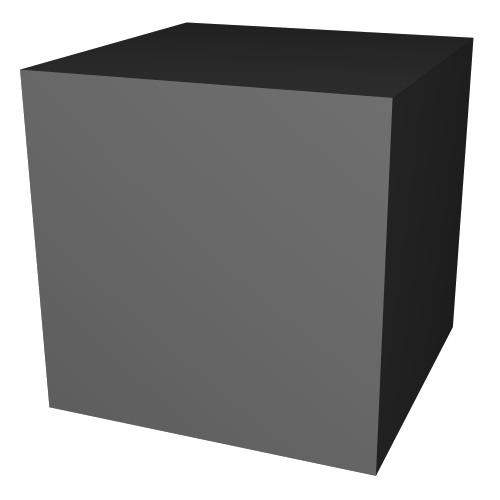
\includegraphics[width=\textwidth]{img/maya0.png}
        \end{subfigure}%
        ~ % use \qquad??
        \begin{subfigure}[t]{0.3\textwidth}
                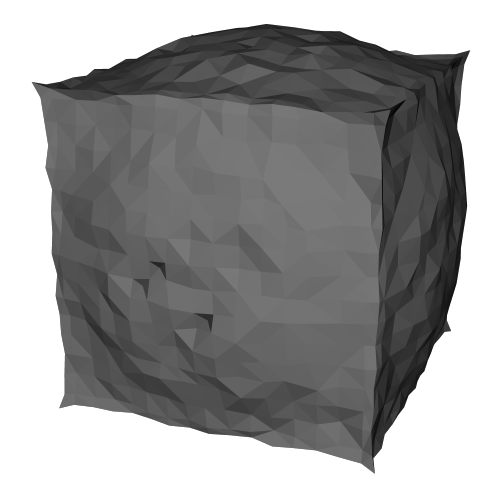
\includegraphics[width=\textwidth]{img/maya1.png}
        \end{subfigure}

        \begin{subfigure}[t]{0.3\textwidth}
                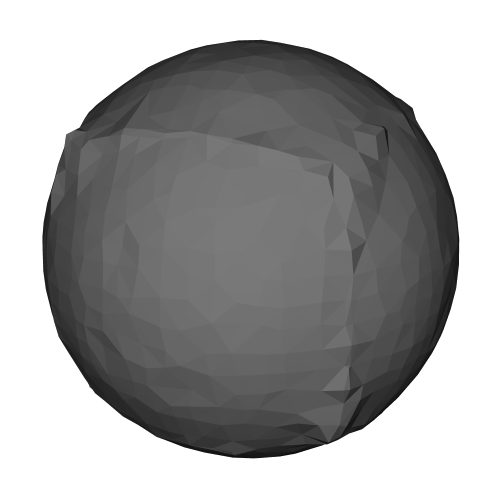
\includegraphics[width=\textwidth]{img/maya2.png}
        \end{subfigure}%
        ~ % use \qquad??
        \begin{subfigure}[t]{0.3\textwidth}
                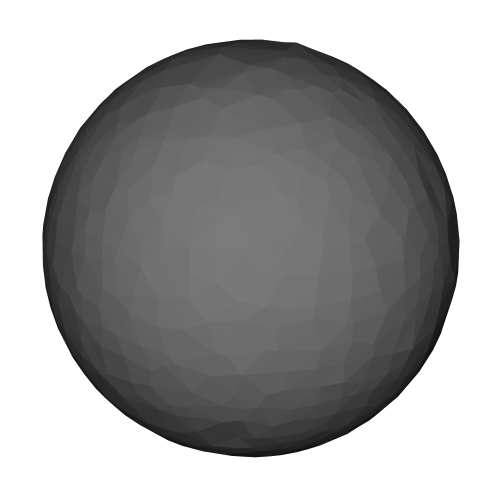
\includegraphics[width=\textwidth]{img/maya3.png}
        \end{subfigure}
        \caption{Pictures of four different stages in the simulation process using
                 the visMesh plugin.}
        \label{fig:vismesh}
\end{figure}
\end{frame}

\begin{frame}
    \frametitle{Textures \& Renderes}
    \framesubtitle{Results \& Future}

    \graphicc{0.8}{img/texture.png}{An advanced texture applied to a
      multi body mesh.}{fig:texture}
\end{frame}


\begin{frame}
    \frametitle{Performance \& Memory Load}
    \framesubtitle{Results \& Future}

    \graphicc{0.8}{img/cubeFine.png}{The memory load of the plugin during
      simulation}{fig:memory}
\end{frame}

\begin{frame}
    \frametitle{What's next?}
    \framesubtitle{Results \& Future}
    \vspace*{\fill}
    \begin{itemize}
      \item Implement uniform mesh storage
      \item Easier usage
      \item New parametertypes
      \item Saveability
    \end{itemize}
    \vspace*{\fill}
\end{frame}

\section{Demonstration \& Questions}

\begin{frame}
    \frametitle{Demonstration \& Questions}
    \vspace*{\fill}
    If there is time: Demo video.

    \noindent Else: Questions.
    \vspace*{\fill}
\end{frame}

\end{document}